\section{Background}
\label{sec:kv_model}

In this section, we discuss \KVS\ internals that serve us in the
remainder of the paper.  We abstract from any particular store, focus
on main concepts, and ground concepts in existing \KVSs\ such
as~\cite{chang:bigtable, decandia:dynamo, cooper:pnuts, george:hbase,
  hewitt:cassandra}. We only consider the highly distributed stores
that have emerged over the last decade and disregard centralized
\KVSs.  Our objective is to distil a set of features our
\VMS\ requires from a \KVS. In the second part of the section we 
discuss the consistency model. We establish a notion to describe
tables and records in the system. Further, we constrain the relations 
between tables in order to express a certain level of consistency. 




% As \HB\ is modelled after \BT, and
%\CAS\ combines features of \DY\ and \BT, we restrict our discussion
%below to \HB, \CAS, and \PN.

\subsection{KV-store Design Overview}

In the upper half of 
Figure~\ref{fig:kv_model} you can see our generalized \KVS\ model. 
Some \KVSs\ explicitly designate a master node, e.g., \HB\ or \BT,
while others operate without explicit master, e.g., \CAS, where a
leader is elected to perform management tasks, or \PN, where
mastership varies on a per-record basis.  In all cases, a system
\textit{node} represents the unit of scalability: The number of nodes
can vary to accommodate load change.
Nodes persist the data stored in the system. In contrast to a
centralized SQL-based DBMS, a node manages only part of the overall
data (and part of the request load).

A \textit{file system} builds the persistence layer of a node in a
\KVS. For example, \HB\ stores files in the Hadoop distributed file
system (HDFS). \CAS\ and \PN\ resort to node-local file systems for
storage and do not rely on a distributed file system.

Whereas, \HB\ relies on HDFS for redundancy of data, \CAS\ relies on
its own replication mechanism to keep data highly available in face of
failures.  If a node crashes, replicas serve to retrieve and restore
data.

A \textit{table} in a \KVS\ does not follow a fixed schema. It stores
a set of table records called \textit{rows}. A row is uniquely
identified by a \textit{row key}. A row can hold a variable number of
\textit{columns} (i.e., a set of column-value pairs). Columns can be
further grouped into \textit{column families}. Column families provide
fast sequential access to a subset of columns. They are determined
when a table is created and affect the way the \KVS\ organizes table
files.

\textit{Key ranges} serve to partition a table into multiple parts
that can be distribute over multiple nodes.  Key ranges are defined as
an interval with a \textit{start} and an \textit{end row key}.
\PN\ refers to this partitioning mechanisms as \textit{tablets}, while
\HB\ refers to key ranges as \textit{regions}. Multiple regions can be
assigned to a node, referred to as a \textit{region server}.  In
general, a \KVS\ can split and move key ranges between nodes to
balance system load or to achieve a uniform distribution of data.

%With regard to key
%range management, a \KVS\ supports the set of events specified in
%Table~\ref{tab:kvs_a_events}.

%
% aj - above - are these events really important for the paper ad
%              the design of VMS? If not, we could do away with
%              them.
%

\begin{figure} 
	\centering 
	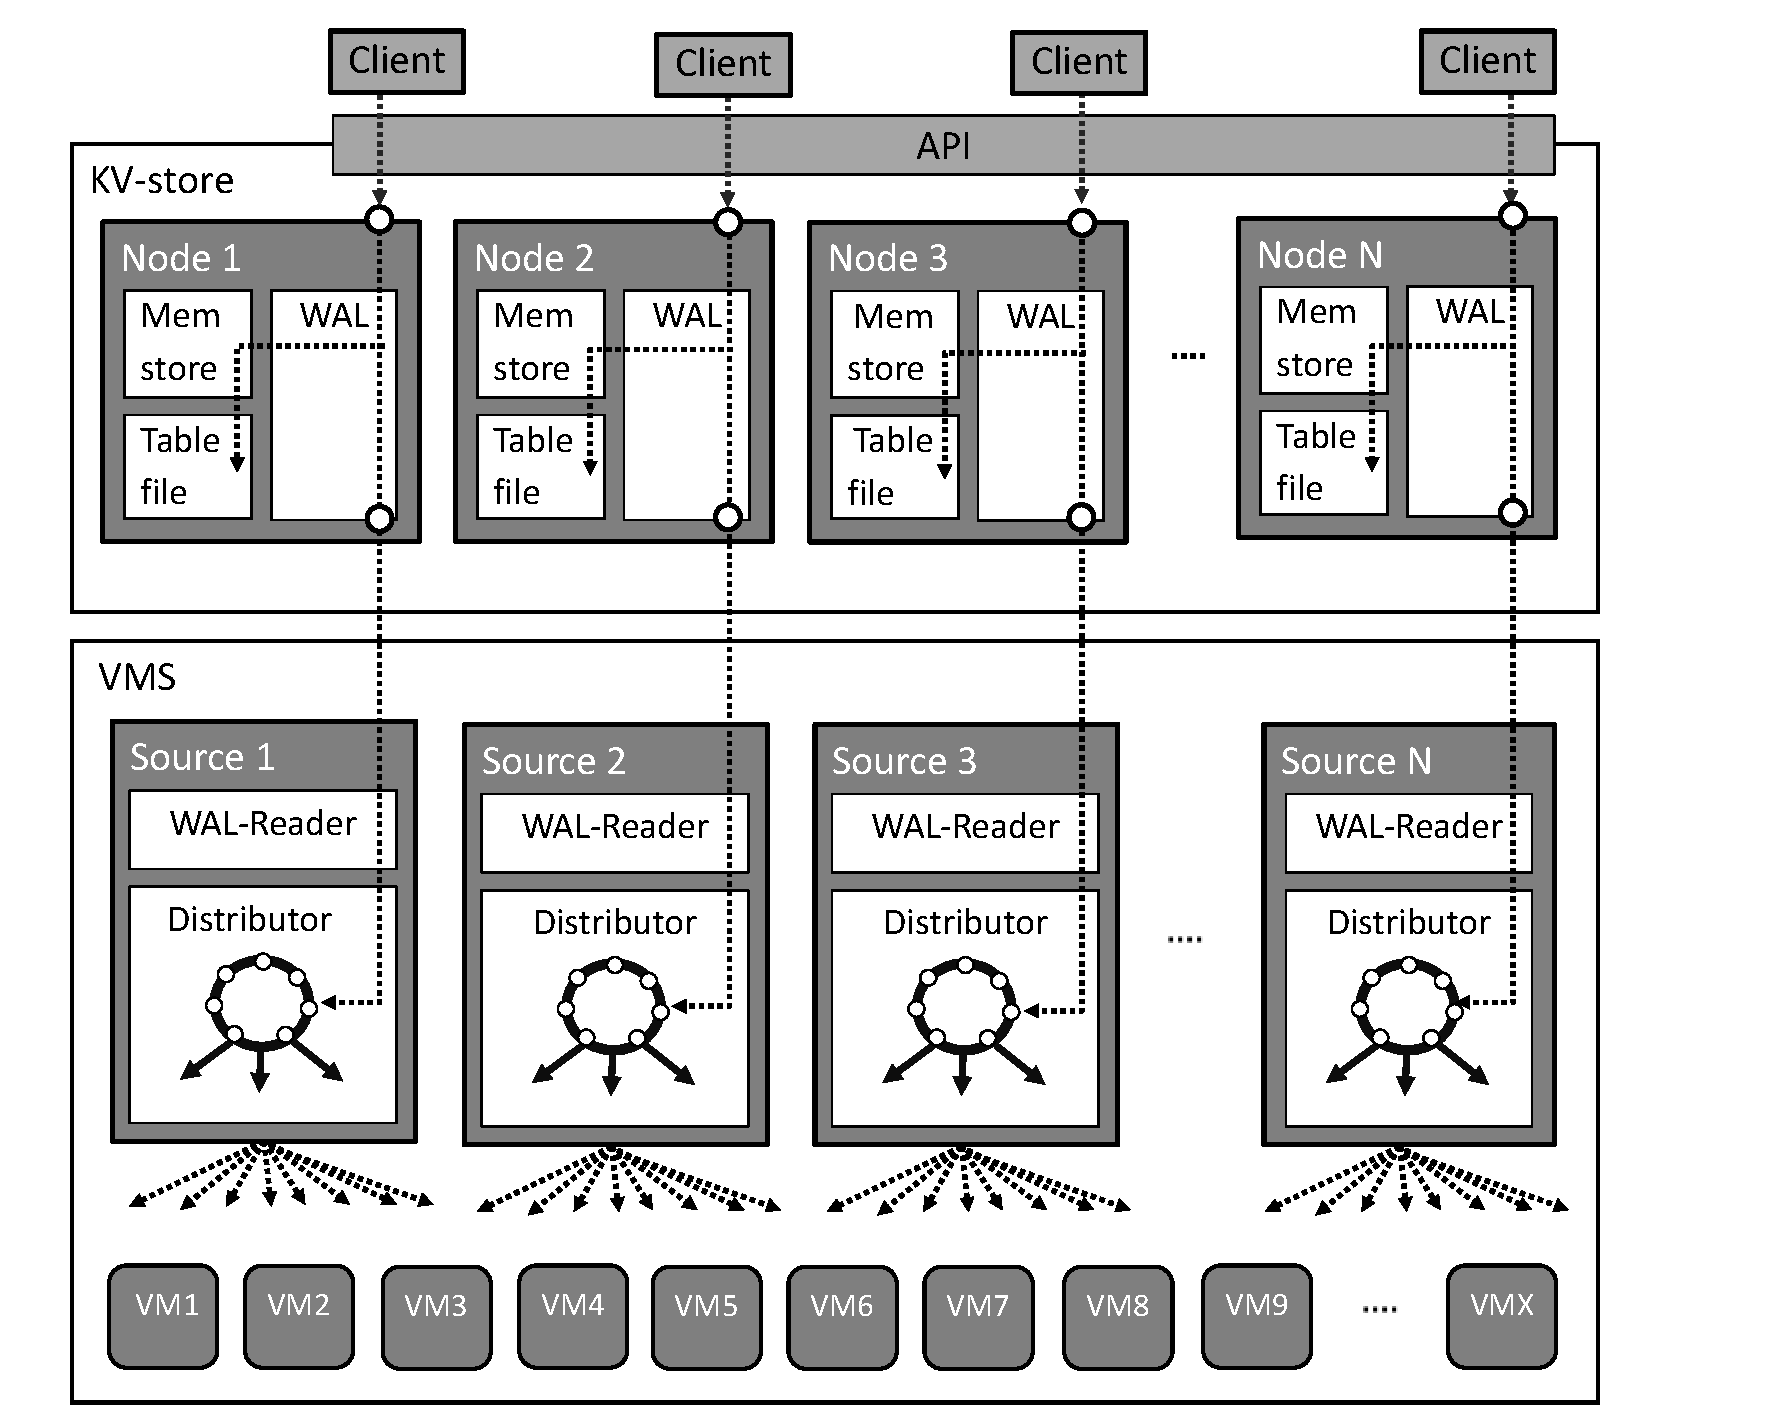
\includegraphics[width=\linewidth]{figures/KVModel} 
	\vspace{-5mm}	
	\caption{KV-Store and VMS} 
	 \vspace{-4mm}
	\label{fig:kv_model} 
\end{figure} 

\textbf{Read/Write Path} -- The \KVS\ API supports three client-side \textit{operations}:
\textit{put}, which inserts a record, \textit{get}, which retrieves a
record, and \textit{delete}, which removes a record\footnote{Sometimes
  there are additional methods, e.g., a range scan or passing a
  selection predicate to the store. However, none of them extends
  beyond repeated single row access; none of them offers expressive
  semantics.}.

In the read/write path, when reading or updating a table record,
requests pass through as few nodes as possible to reduce access
latency.  Also, a \KVS\ aims to distribute client requests among all
system nodes to spread load. For example, \HB\ routes client requests
from a root node down to the serving node in a hierarchical
manner. \CAS, on the other hand, lets clients connect to an arbitrary
node which forwards the request to the serving node. In either case,
the clients ends up at one particular node that is serving the key range
the client wants to access.


Every node maintains a \textit{transaction log} (\TL), referred to a
write-ahead log in \HB\ and commit log in \CAS.  When a client
operation arrives, it is first written into the \TL\ of the node
(cf. Figure~\ref{fig:kv_model}). From then on, the operation is
durably persisted.  Subsequently, the operation is inserted into a
\textit{memstore}.  Memstores are volatile; upon node crash, they are
recovered from the \TL, which contains the operation sequence a node
saw over time.  During recovery, this sequence is replayed from the
log. Once a memstore exceeds a set capacity, it is flushed to disk.
Continuous flushes produce a set of table files, which are
periodically merged by a compaction process. After a flush, the
corresponding entries in the \TL\ are purged.

%\subsection{KV-store Data Model}
%
%The data model of a \KVS\ differs from that of a relational DBMS.  We
%propose a model that is representative for today's \KVSs. The model
%serves throughout the paper to help specify views and view update
%programs. Typically, \KVSs\ do not required fixed data schemas, but
%rather accommodate dynamic schema changes.
%
%Thus, we formalize the data model of a \KVS\ as a map of key-value
%pairs $\{\langle k_1, v_1\rangle,..,\langle k_n,v_n\rangle\}$
%described by a function $f:K \rightarrow V$. Systems like \BT,
%\HB\ and \CAS\ established data models that are multi-dimensional maps
%storing a row together with a variable number of columns per row. For
%example, the 2-dimensional case creates a structure
%$\{\langle(k_1,c_1),v_{1,1}\rangle,\langle (k_n,c_n)
%,v_{n,n}\rangle\}$ with a composite key $(k_n,c_n)$ that maps to a
%value $v_{n,n}$ described by $f:(K,C)\rightarrow V$. In the
%3-dimensional case, another parameter, a timestamp, for example, is
%added to the key, which may serve versioning purposes. For this paper,
%the 2-dimensional model suffices.\footnote{Our approach also works
%  with the 1-dimensional case, which is representative for simple
%  key-blob stores.  We use the 2-dimensional case, here, as it is more
%  expressive.}
%
%We denote a table by $A = (K, F)$, where $K$ represents the row key
%and $F$ a \textit{column family}. Column families are defined when a
%table is created. They are used in practice to group and access sets
%of column-value pairs. In terms of our data model, column families are
%optional. They can be dynamically assigned as the row is created. Let
%a base table row $a \in A$ be defined as $a=(k,\{\langle
%c_1,v_1\rangle..\langle c_n,v_n\rangle\})$. In this notation, the row
%key $k$ comes first, followed by a set of column-value pairs
%$\{\langle c_1,v_1\rangle..\langle c_n,v_n\rangle\}$ belonging to the
%column family. This notation more closely resembles a database row and
%is used throughout the remainder of this paper. When using multiple
%column families, we define a table as $A = (K, F_1,...F_n)$. Then, the
%assignment of a column-value set to a column family $F_x$ is denoted
%by $\{..\}_x$. The corresponding row would be defined as $a=(k,
%\{\langle c_1,v_1\rangle..\langle c_i, v_i\rangle\}_1..., \{\langle
%c_{i+1},v_{i+1}\rangle.. \langle c_n,v_n\rangle\}_n)$.




\textbf{Extension points} -- We designed \VMS\ to react to \KVS\ events and to not interfere with
store-internal read/write paths for data processing. In this spirit,
we determined a number of common ``extension points,'' all considered
\KVSs\ exhibit.  We characterize extension points by events, which the
\VMS\ reacts to in maintaining views.  There are two different kinds
of events that \VMS\ needs to react to: \textit{administrative events}
and \textit{data events}.

Administrative events occur during a state change in the
\KVS\ infrastructure, e.g., a new node is added (and starts processing
client operations).  \KVSs\ provide different ways to react to
administrative events. For example, \HB\ lets developers use various
kinds of \textit{coprocessors}, which refer to application-developer
provided code pieces that can be deployed and run on system nodes
before or after certain events. We leverage this mechanisms to notify
\VMS, as soon as certain events of interest occur (e.g., the addition
of a node.)  \VMS\ reacts accordingly and allocates resources to
maintain view tables that depend on the newly added node.

%\begin{table}[h]
%\rowcolors{2}{gray!10}{gray!30}
%\setlength{\belowrulesep}{0pt}
%\setlength{\aboverulesep}{0pt}
%\setlength\extrarowheight{2pt}
%\begin{center}
%\begin{tabular}{l l l}
%\toprule
%Component & Event & Method \\
%\midrule
%Node       & added         & \textit{onNodeAdded()}  \\
%           & removed       & \textit{onNodeRemoved()}    \\
%Key-range  & opened        & \textit{onKeyRangeOpened()}\\
%           & closed        & \textit{onKeyRangeClosed()} \\
%           & split         & \textit{onKeyRangeSplit()} \\
%           & moved         & \textit{onKeyRangeMoved()} \\
%%Transaction log & replay & \textit{onTLReplay()}\\
%% & purge & \textit{onTLpurge()} \\ 
%\bottomrule 
%\end{tabular}
%\caption{Administrative events}
%\label{tab:kvs_a_events}
%\end{center}
%\end{table}


Data events occur, when a client updates a base table (e.g., put,
delete). Consequently, base table derived view tables become stale and
\VMS\ needs to update them. Generally speaking, there are three
methods to stream updates on base data from the \KVS\ to \VMS: (1)
Access the store's API, (2) intercept operations (e.g., via
coprocessors), (3) read the \TL.

Method~1 may lead to inconsistent view states, as base data 
change, before a prior update can be retrieved; none of the popular
\KVSs\ offers snapshot isolation. Also, this method would incur a lot
of overhead (e.g., an update would trigger a read and one or more
write to update derived views.)  Method~2 looks promising, especially,
with regard to freshness of the view (coprocessor execution is
synchronous in the update path), but it is only suitable if the number
of maintained views is small, otherwise \KVS\ operations would be
needlessly delayed, counter-acting the asynchronous operation behind
many design decisions. Thus, Method~3 is the preferred choice.

Method~3 has several benefits: (i) Reading \TL\ is asynchronous and
decouples processing. It neither interferes with update processing,
i.e., no latency is added into the update path, nor imposes additional
load.\footnote{Our experiments confirmed that the penalty of reading
  from the file system are far smaller than intercepting events.} (ii)
Moreover, maintaining numerous views at once means that every base
table operation generates multiple view updates. Using \TL, we
decouple view update from client operation. (iii) Operations in
\TL\ are durably persisted and can be recovered by \VMS. (iv) The 
\TL\ contains operations, not table rows, which is fine for 
incremental maintenance.



%The \KVS\ writes operations, that is client requests, to the \TL, but
%not entire table rows.  In contrast, a table row stores the row state,
%which may result from multiple client requests.  Then, an operation $t
%\in T$ can easily be defined over table row $a \in A$, with $T =
%type(A)$ and $type \in \{put, delete\}$. A put operation in the
%\TL\ is denoted as $t=put (k, \{\langle c_1,v_1\rangle..\langle
%c_n,v_n\rangle\})$. A put inserts or updates the column values at the
%specified row key. A delete operation $t \in T$ is defined as
%$t=delete (k, \{\langle c_1,\emptyset\rangle..\langle
%c_n,\emptyset\rangle\})$.  Note that we are leaving the values empty;
%the client just specifies the row key and columns that are to be
%deleted. A stream that is the output of one node's \TL\ is denoted as
%a sequence of operations $ts \in TS=(T_1,..,T_n)$. Finally, we can
%define the complete output of the \KVS\ as a set of operation streams
%as $ts_1,..ts_n \in TS$.

%
% aj - above - should we outline the difficulties imposed by not
%              having the values avail. for a delete?
%              Not mission critical.


\subsection{Consistency model}
\label{subsec:consistency_model}

A view data consistency model\footnote{Not to be confused with consistency models
for transaction processing (i.e. system-centric and client-centric models)} 
validates the correctness of a view 
table. Furthermore, the model evaluates a view table's ability to follow 
a sequence of base table states an produce a corresponding number of 
valid view states. It does so by defining different levels of 
consistency of a view~\cite{zhuge:view, wang:efficient, zhang:parallel, 
zhuge:strobe, jacobsen:viewmaintenance}. Depending on view types, view 
maintenance strategies, and view update programs, none, some, or all of 
the levels are attainable~\cite{zhuge:view, wang:efficient, 
zhang:parallel, zhuge:strobe, jacobsen:viewmaintenances}. 

\setlength{\abovedisplayskip}{5pt}
\setlength{\belowdisplayskip}{5pt}

As base and view table are nothing more than standard tables in the \KVS, 
we create a notion of tables and records first. The data model of a \KVS\ 
differs from that of a relational DBMS.  We propose a model that is representative for today's \KVSs. We 
formalize the data model of a \KVS\ as a map of key-value
pairs $\{\langle k_1, v_1\rangle,..,\langle k_n,v_n\rangle\}$
described by a function $f:K \rightarrow V$. Systems like \BT,
\HB\ and \CAS\ established data models that are multi-dimensional maps
storing a row together with a variable number of columns per row. For
example, the 2-dimensional case creates a structure described by 
$f:(K,C)\rightarrow V$ where $K$ is the row key and $C$ is the column key. 
In the 3-dimensional case, another parameter, a timestamp, for example, is 
added to the key, which may serve  versioning purposes. For this paper, 
the 2-dimensional model suffices. This notation more closely resembles a 
database row and is used throughout the remainder of this paper. We use the 
following notation to define: (a) a table (with $K$ being the row key and
$F$ being a set of column-value pairs), (b) a record, (c) a put operation 
and (d) a delete operation.
%\footnote{Our approach also works
%  with the 1-dimensional case, which is representative for simple
%  key-blob stores.  We use the 2-dimensional case, here, as it is more
%  expressive.}
\begin{align*}
 	(a)&\enspace T=(K, F)\\
 	(b)&\enspace r=(k,\langle c_1,v_1\rangle..\langle c_n,v_n\rangle)\\
 	(c)&\enspace p=put(k,\langle c_1,v_1\rangle..\langle c_n,v_n\rangle)\\
 	(d)&\enspace d=del(k)
\end{align*}



%When using multiple
%column families, we define a table as $A = (K, F_1,...F_n)$. Then, the
%assignment of a column-value set to a column family $F_x$ is denoted
%by $\{..\}_x$. The corresponding row would be defined as $a=(k,
%\{\langle c_1,v_1\rangle..\langle c_i, v_i\rangle\}_1..., \{\langle
%c_{i+1},v_{i+1}\rangle.. \langle c_n,v_n\rangle\}_n)$.

Lets now define a base table as $B=(K,F)$ and a view table
as $V=(K,F)$. The relation between both tables can be expressed as
$View(B)=V$, where function $View$ can be any term described by
relational algebra (e.g. view table is a projection of base table, 
$V=\pi_{c_1}(B)$). If the clients of the \KVS\ start doing their updates, 
the state of the base table changes; we depict the sequence of states 
with indices $B_0..,B_i,..,B_f$, where $B_0$ is the initial state, $B_i$ is an
arbitrary intermediate state and $B_f$ is the final state. Every client
put or delete operation causes a record to change its version (all versions
of a record are called a record's timeline) and thus,
the base table to change its state. Two states can be compared by the 
operator $\leq$. $B_i \leq B_j$ means that the versions of all records in 
$B_j$ are equal or newer than the versions of records in $B_i$. 

Once the base table changes, the view table -- or rather the system that
maintains the view -- needs to react and in-cooperate the changes into 
the view. How accurate this maintenance is done, is defined by the 
following levels:



\begin{enumerate}
 \setlength{\itemsep}{5pt}
\item[]\textit{Convergence:} A view table converges, if after the system
  quiesces, the last view state $V_f$ is computed correctly. This
  means it corresponds to the evaluation of the view expression over
  the final base state $V_f=View(B_f)$. View convergence is a minimal 
  requirement, as an incorrectly calculated view is of no use.

\item[]\textit{Weak consistency:} Weak consistency is given if the view
  converges and all intermediate view states are valid, meaning that
  there exists a base table state in the sequence of base table states
  produced by the operation sequence from which they can be derived
  %$V_j=View(B_i)$.

\item[]\textit{Strong consistency:} Weak consistency is achieved and the
  following condition is true. All pairs of view states $V_i$ and
  $V_j$ that are in a relation $V_i \leq V_j$ are derived from base
  states $B_i$ and $B_j$ that are also in a relation $B_i \leq B_j$.

\item[]\textit{Complete consistency:} Strong consistency is achieved
  and every base state $B_i$ of a valid base state sequence is
  reflected in a view state $V_i$. Valid base state sequence means
  $B_0 \leq B_i \leq B_{i+1}\leq B_f$.
\end{enumerate}


\noindent
\textit{Example~1:} Imagine a base table $B=(K, F)$ and a view table 
$V=\gamma_{c_1, sum(c_2)}(B)$. The initial state of the base table is 
$B_0=\{(k_1,\langle c_1,x_1\rangle, \langle c_2,15\rangle)\}$ and the 
corresponding state of the view table is $V_0=\{(x_1, \langle c_{sum},15\rangle)\}$. Now, the following 
update operations are applied to the base table: 
\begin{align*}
	(1)\enspace &put(k_1,\langle c_1,x_1\rangle, \langle c_2,20\rangle)\\
	(2)\enspace &put(k_2,\langle c_1,x_1\rangle, \langle c_2,10\rangle)\\
	(3)\enspace &del(k_1)\\
	(4)\enspace &put(k_3,\langle c_1,x_1\rangle, \langle c_2,45\rangle)
\end{align*}

\noindent
The base table reaches a final state 
$B_f=\{(k_2,\langle c_1,x_1\rangle, \langle c_2,10\rangle),\linebreak (k_3,\langle c_1,x_1\rangle, \langle c_2,45\rangle)\}$. 
Accordingly, to achieve consistency level convergence, the maintenance 
system has to compute the final view state as: 
$V_f=\{(x_1, \langle c_{sum},55\rangle)\}$. To
achieve weak consistency the maintenance system could (there are various
possibilities) produce two intermediate view states 
$V_1=\{(x_1, \langle c_{sum},30\rangle)\}$ and 
$V_2=\{(x_1, \langle c_{sum},20\rangle)\}$. Note
that, though both states are valid, they are not in correct order. Thus,
to achieve strong consistency the order of view states $V_1$ and $V_2$ has
to be changed. The last (and usually too costly) level, complete consistency,
can be achieved, representing all intermediate base states in the view:
$V_1=\{(x_1, \langle c_{sum},20\rangle)\}$, $V_2=\{(x_1, \langle c_{sum},30\rangle)\}$ 
 and $V_3=\{(x_1, \langle c_{sum},10\rangle)\}$ 



A system that is to achieve a given consistency level has to offer
certain guarantees based on which the consistent and correct
materialization of views can be based.\\


\newtheorem{theorem}{Theorem}
\noindent
\begin{theorem}
\label{theo:strong_consistency}
The following requirements are sufficient to guarantee that views are
maintained \textit{strongly} consistent in VMS.

\begin{align*}
	1.\enspace&\text{View updates are applied \textit{exactly once}}\\
	2.\enspace&\text{View updates are \textit{atomic}}\\
	3.\enspace&\text{(Base-)record \textit{timeline} is always preserved}
%	\item  View records are processed \textit{locally}
\end{align*}
\end{theorem}
\hfill \newline
Due to the space constraints, we present the theorem without proof.
(We refer the reader to \cite{extended:version} for the complete proof.)
Instead we provide a brief explanation of Theorem~1. If we make use of 
Rule~1 of the theorem, we make sure that all update operations are delivered and 
applied exactly once. Rule~1 alone does not guarantee convergence
of the view. When using parallel execution e.g., multiple update operations 
might be applied to the same view record concurrently and change its 
correctness.

\noindent
\textit{Example~2:} We reconsider the table set-up of Example~1 and its
update operations (1) - (4). When two update programs process update operation
(1), and (2) in parallel, the following can happen: Update program~1 and
Update program~2 retrieve the initial view record 
$(x_1, \langle c_{sum},15\rangle)$ simultaneously from the view. Update 
program~1 applies its incremental update, leading to a new view record 
$(x_1, \langle c_{sum},20\rangle)$ and writes it back to the view; 
update program~2 also applies its incremental update to the initial 
value, leading to $(x_1, \langle c_{sum},25\rangle)$ and writes back to 
the view. The result is an incorrect value, as both incremental updates
should be applied subsequently, leading to a view record 
$(x_1, \langle c_{sum},30\rangle)$.

Rule~2 -- more specifically the isolation of transactions -- would have
prevented the wrong execution in Example~2. If Rule~1 and Rule~2 of the
theorem are applied, convergence is still not guaranteed. Asynchronous
processing and high parallelism can lead to reordering of update 
operations. 

\noindent
\textit{Example~3:} Again, we consider table set-up of Example~1 and 
operations (1) - (4). Operation (3) and operation (1) touch the
same base table key $k_1$; if their order is changed, meaning (3) is 
processed before (1), the end result is incorrect. Exchanging the order 
of a put and a delete operation, causes the value of this particular 
row-key to be present in the view computation, where it shouldn't. 

Therefore, we also apply Rule~3 and demand the preservation of a record's
timeline. All three rules together make sure that convergence weak and 
even strong consistency (correct ordering is established) can be achieved. 
By complying to the requirements of the theorem, we show that our approach 
can attain strong consistency for the views it maintains.






%
%In our context, we stream operations from multiple 
%sources (i.e. nodes) and apply them to different parts of the view 
%table, located on different nodes. We want to parallelize view 
%maintenance and improve performance to a great extent, we further relax 
%the consistency model. We do not claim the stream of a local source to 
%be in sequence. Instead, we define consistency on a record base level. 
%Every sequence of operations, that is applied to a specific row key has 
%to be in sequence. A base state $B_j$ is said to be greater than $B_i$ 
%if all operations to a specific row key in $B_i$ are included in $B_j$ 
%plus a number of subsequent operations. Formally we write $(\exists t_k 
%\in B_j)(\forall t_l \in B_i)\;k > l\;\land\; r(t_k)=r(t_l)$. Function 
%$r()$ delivers, when applied to an operation, the row key of that 
%operation. Now, we define consistency levels in agreement to the 
%model. Formally, the consistency levels of the model are 
%defined as follows:

